\chapter{Developed System}

	In previous sections of this documents, I have explained the main idea of the project, and what technologies are going to be used to develop a fully functional system. Just to remember, the objective of the project is to perform a Pick and Place task using a Universal Robots' UR3 robotical arm.
	
	The objects have to be taken from a box (Environment Box) and placed in another box (Place box). The pieces had to be something light due to the limitations of the UR3 robot that we commented before. As there wasn't any sponsor for the project we could decide the shape of the pieces, and we decided to use 5 cm size wooden squares as the ones showed in \autoref{fig:pieces}.
	
	\begin{figure}[h]
		\centering
		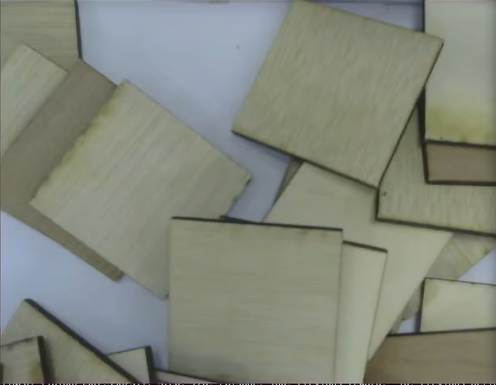
\includegraphics[width=0.7\linewidth]{Images/pieces}
		\caption[pieces]{Wooden Pieces used in the project}
		\label{fig:pieces}
	\end{figure}
	
	\section{Hardware Architecture}
	
		In order to make this system work, we need a really complex architecture that can be split in three different categories. These categories are:
		
		\begin{itemize}
			\item[\textendash]Environment
			\item[\textendash]sensorimotor devices
			\item[\textendash]Computational devices
		\end{itemize}
	
		To understand it better, we are going to use \autoref{fig:imagen-arquitectura} and \autoref{fig:imagen-arquitectura-ii}, which are labeled pictures of the architecture, where we are going to be able to see how the components of the architecture are like. 
		
		\begin{figure}[H]
			\centering
			\includegraphics[width=0.9\linewidth]{"Images/Imagen Arquitectura"}
			\caption[Picture of Architecture I]{Labelled picture of the Architecture I}
			\label{fig:imagen-arquitectura}
		\end{figure}
	
		
		\begin{figure}[H]
			\centering
			\includegraphics[width=0.9\linewidth]{"Images/Imagen Arquitectura II"}
			\caption[Picture of Architecture II]{Labelled picture of the Architecture II}
			\label{fig:imagen-arquitectura-ii}
		\end{figure}
	
		In the pictures we can see multiple elements tagged with different colours and labels. Each colour represents a category. 
		
		
		The environment elements, that can be found in green, and labelled with EN, are basically all the things that the robot will have to interact with. The sensorimotor elements, that can be found in orange and with the label SM, are all the elements needed to allow the robot interact with the environment. And finally, in blue and with label CP, we can find the computational elements, which are the ones used to receive all the sensor information, decide which movement to do, and communicate with the robot and the gripper for them to actually perform these actions.
		
		But, what are all these elements? Let's explain them:
		
		\begin{itemize}
			\item[\textendash]\textbf{Environment}: We can see this elements in both images, from different perspective.
			\begin{itemize}
				\item[\textendash]\textbf{EN1}: The Environment box where the agent has to take the pieces
				\item[\textendash]\textbf{EN2}: The box where the agent has to place the pieces
			\end{itemize}
			\item[\textendash]\textbf{Sensorimotor devices} Ones are showed in one image, and others in the other.
			\begin{itemize}
				\item[\textendash]\textbf{SM1}: This is the Onboard camera, used for the agent to decide which action to take. It is attached to the gripper, so in the picture they are shown together.
				\item[\textendash]\textbf{SM2}: Together with the camera, we can see the "Home made" gripper used to pick the pieces.
				\item[\textendash]\textbf{SM3}: the upper camera, where the agent can pick a global picture of the environment. This picture will be important, but we will explain it later.
				\item[\textendash]\textbf{SM4}: the pump of the Gripper.
				\item[\textendash]\textbf{SM5}: Both 12V and 24V power adaptor used to feed the pump and some sensors.
			\end{itemize}
			\item[\textendash]\textbf{Computational devices}. In the picture we cannot see all the computer used in the project, but there are 2 icons used to represent  them.
			\begin{itemize}
				\item[\textendash]\textbf{CP1}: This is the ROS Master Node. All of the nodes of the system will be connected to this node. Besides being the master node, robot\_controller node and Universal Robots driver will also bo running in this computer.
				\item[\textendash]\textbf{CP2}: This computer is a really powerful one, with one of the bes graphical cards in the market an 32 GB of RAM. It will be used to train the algorithm, running the ai\_manager node.
				\item[\textendash]\textbf{CP3}: This mini-computer can be seen in one of the pictures and its a Raspberry-pi. This computer will be used as a bridge form the arduino card of the gripper and the ROS master node. The cameras will also be attached to the Raspberry-pi.
			\end{itemize}
		\end{itemize}
	
	\section{Logical Architecture}
		
		Once we have seen the physical architecture of the project, let's see how the Software architecture is. The Logical architecture will use all the elements commented on the previous section, and they will work together using ROS (Robot Operative System). 
		
		\begin{figure}
			\centering
			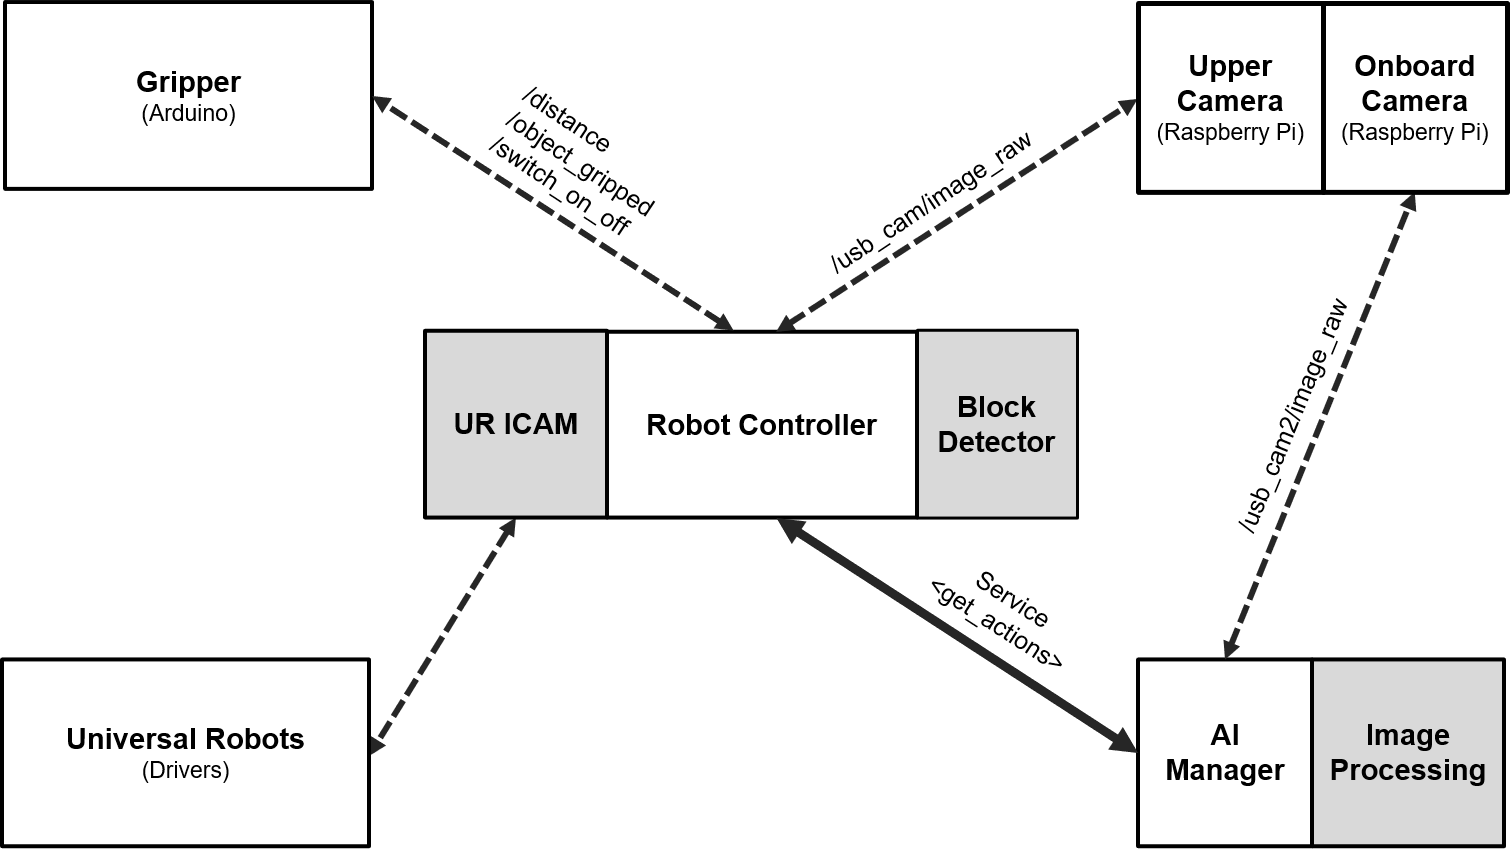
\includegraphics[width=0.7\linewidth]{Images/Architecture}
			\caption[Logical Architecture]{Logical Architecture of the project}
			\label{fig:architecture}
		\end{figure}
	
		In \autoref{fig:architecture} we can see the logical architecture of the application, which is composed of 6 nodes communicating one with each other. We can see that the communication topics are written in the figure and that there are some squares attached one to another, and some of them are grey. All the white squares are ROS nodes, while grey ones are separate pieces of code that the nodes are using, but they are not ROS nodes by themselves. On the other hand, both camera nodes that are together in the upper right corner are two independent nodes, but using the same code to send the cameras images.
		
		To explain briefly what every node does, probably it is easier going step by step from the simplest architecture to the final one, so that we see what every node is doing.
		
		\begin{figure}[H]
			\centering
			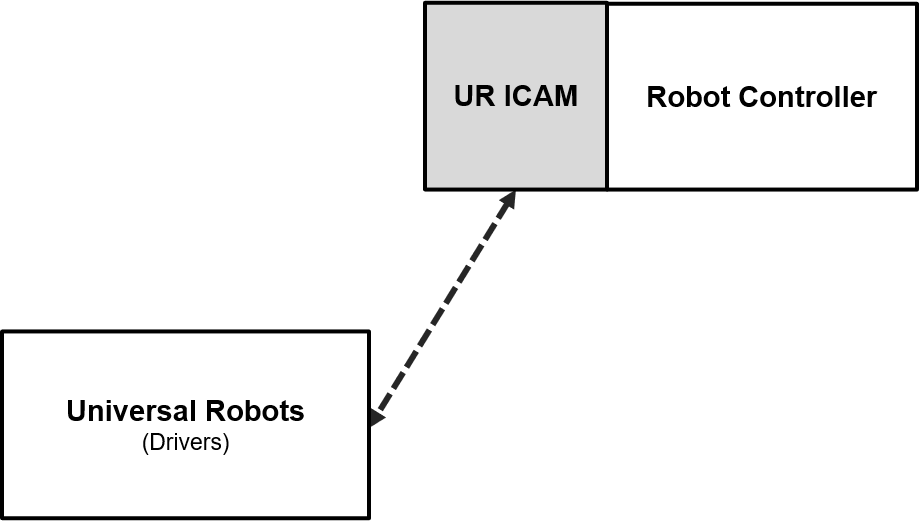
\includegraphics[width=0.7\linewidth]{Images/ArchitectureI}
			\caption[Architecture I]{From the simplest to the final Architecture I}
			\label{fig:architecturei}
		\end{figure}
	
		In \autoref{fig:architecturei}, there are only three components. However, Both Universal Robots Drivers and UR ICAM were not developed by us and are like black-boxes for us. That is the reason why there are no ROS topics written in the communication the figure.
		
		Universal Robot Drivers is the one that actually communicates with the robot, and provides all the basic tools needed to control it remotely. On the other side, UR ICAM node is a node developed in the university, and it provides us some methods to control easier the robot. These methods are a personalization of the ones provided by MoveIt library, and they make us possible to go to some angular coordinates of the robot without calculating the optimal path to reach this position, or the same thing with some cartesian coordinates.
		
		Finally, the Robot Controller node is the one that actually is communicating with all the othe nodes of the architecture. All the actions that the robot will be able to perform are here, so just with Robot Controller node we could almost be able to implement a silly random agent to perform a pick and place task.
	
		\begin{figure}[H]
			\centering
			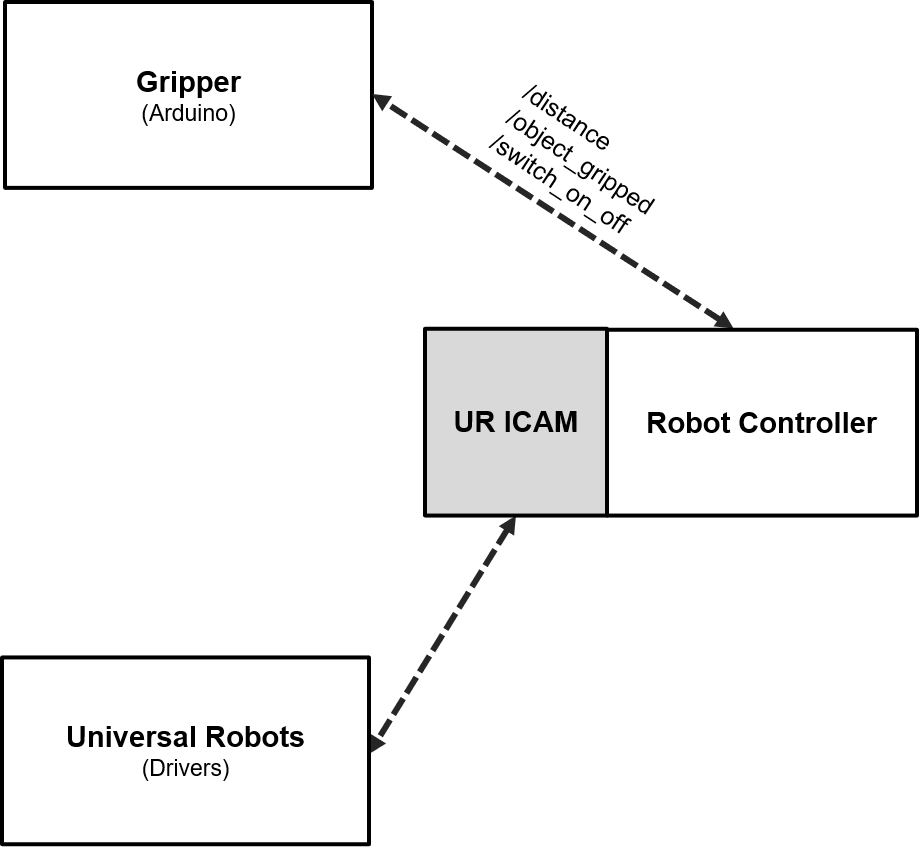
\includegraphics[width=0.7\linewidth]{Images/ArchitectureII}
			\caption[Architecture II]{From the simplest to the final Architecture II}
			\label{fig:architectureii}
		\end{figure}
	
		I said almost, because to perform a pick and place task we also need the gripper node, as we can see in \autoref{fig:architectureii}. This node is running in an ardunio carda communicates by serial port with a Raspberry Pi, which is also connected with the master node. The gripper node uses 3 different topics to communicate with Robot Controller:
		
		\begin{itemize}
			\item[\textendash]\textbf{\textit{\textbackslash distance: }} The gripper is publishing continuously if the gripper is being pushed up or not. Robot Controller wants this information to know when to stop during the pick movement. The Robot basically goes down while \textbf{\textit{\textbackslash distance}} are "False" and stops when they are "True".
			\item[\textendash]\textbf{\textit{\textbackslash switch\_on\_off: }} The gripper listens to this topic. When it receives a "True" message it switch the gripper on, and when it receives a "False" message it switch the gripper off.
			\item[\textendash]\textbf{\textit{\textbackslash object\_gripped: }} The gripper is publishing continuously if there is an object gripped or not. Robot Controller use this information during the pick action. When this action is finished, robot controller checks if an object has been picked or not by reading from this topic. If an object has been picked it goes to the box to place the object and, if not, it just finishes the pick action and request AI Manager for a new action.
		\end{itemize}
	
		\begin{figure}[H]
			\centering
			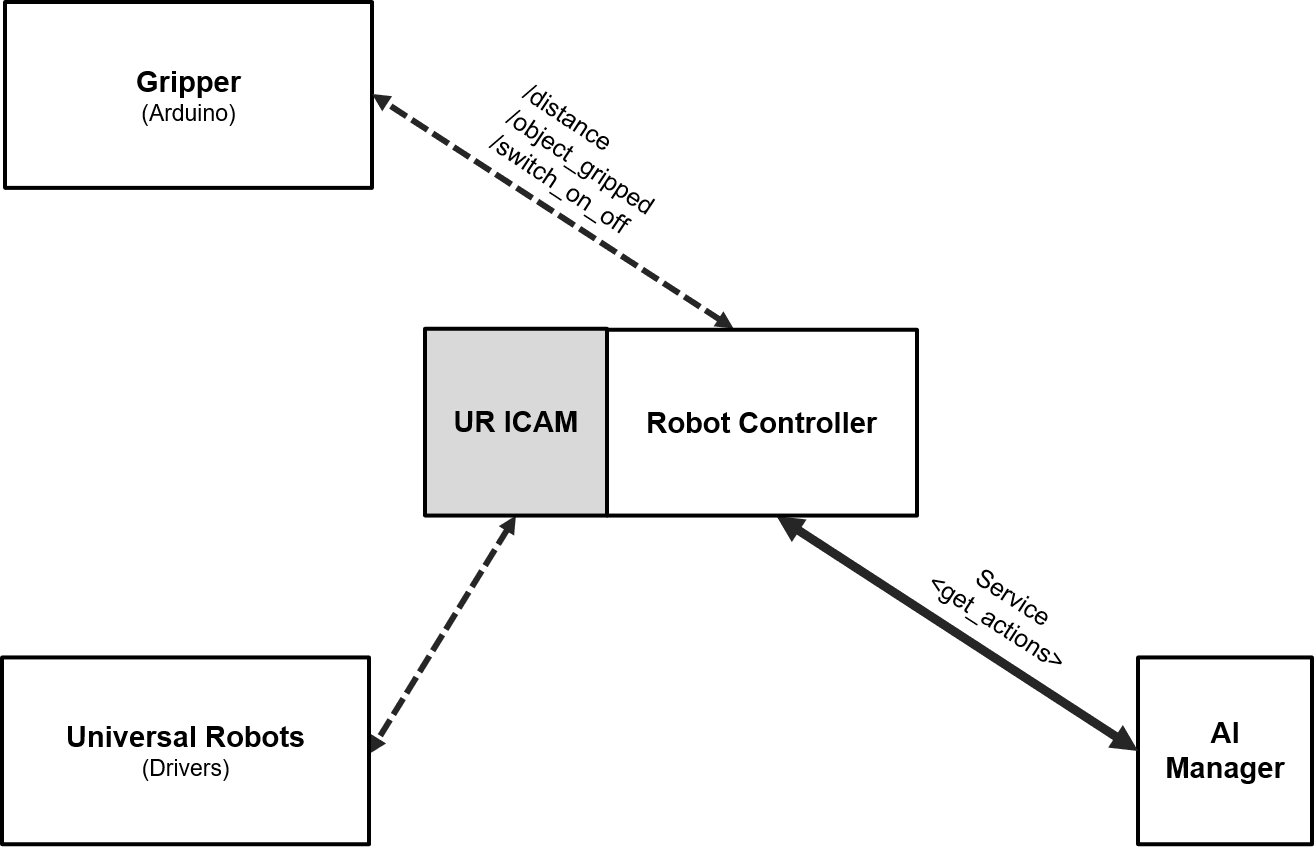
\includegraphics[width=0.7\linewidth]{Images/ArchitectureIII}
			\caption[Architecture III]{From the simplest to the final Architecture III}
			\label{fig:architectureiii}
		\end{figure}
	
		The next step in our trip would be adding the AI Manager Node. This Node is the one who decides which action to perform in each time step. It receives the Coordinate, request an image of the environment (Which in this step is still simulated) and trains a Reinforcement Learning Algorithm to decide which action to perform in each step.		
		
		As we can see in the \autoref{fig:architectureiii}, the arrow representing the communication between Robot Controller and AI Manager is the only continuous line. This is because the communication method is different, in this case we are using ROS Services instead of publishing the messages in topics.
		
		In ROS, the most common way of communicating is using ROS Messages. ROS Messages are simple data structures that are send to a topic, which is basically a queue stored in the Master node. Then, other nodes can be subscribed to this topics so every time that they are free, they ask the master node about the unread messages in the topic. This is called asynchronous communication and, it is probably the best way of sending messages between nodes, because it allows the receiver to adapt its computational needs to the message load received from the topics.
		
		However, in this case asynchronous communication was not possible, because ROS Messages does not ensure the delivery. This was a problem because the Robot Controller could request an action to the AI Manager, and the second one could not receive the message. This is not a problem in this direction because we can solve it by putting a timeout in Robot Controller, and it could make a new request after x time. 
		
		Anyway, this could not be a solution because we need to avoid the AI Manager node to receive the same request twice. This is needed because every time that the AI Manager receives a new action, a new step of the training is performed: A reward is given, random probability decreases, Experience is saved, etc.
		
		ROS Services is the way of performing synchronous communication in ROS, and it ensures that every message is delivered once and only once. AI Manager is though a resting node that does nothing until the Robot Controller nod request an action. It then start calculating the action, trains the net and return the selected action.
		
		get\_actions services is defined by two structures:
		
		\begin{itemize}
			\item[\textendash]Request structure:
			\begin{itemize}
				\item[\textendash]\textbf{x\_coordinate:} X coordinate of the robot used to calculate the reward and training the robot.
				\item[\textendash]\textbf{y\_coordinate:} X coordinate of the robot used to calculate the reward and training the robot.
				\item[\textendash]\textbf{object\_gripped:} Boolean telling whether the robot has an object gripped or not. It is used to calculate the reward of pick actions.
			\end{itemize}
			\item[\textendash]Response structure:
			\begin{itemize}
				\item[\textendash]String telling the action selected
			\end{itemize}
		\end{itemize}
	
		\begin{figure}[H]
			\centering
			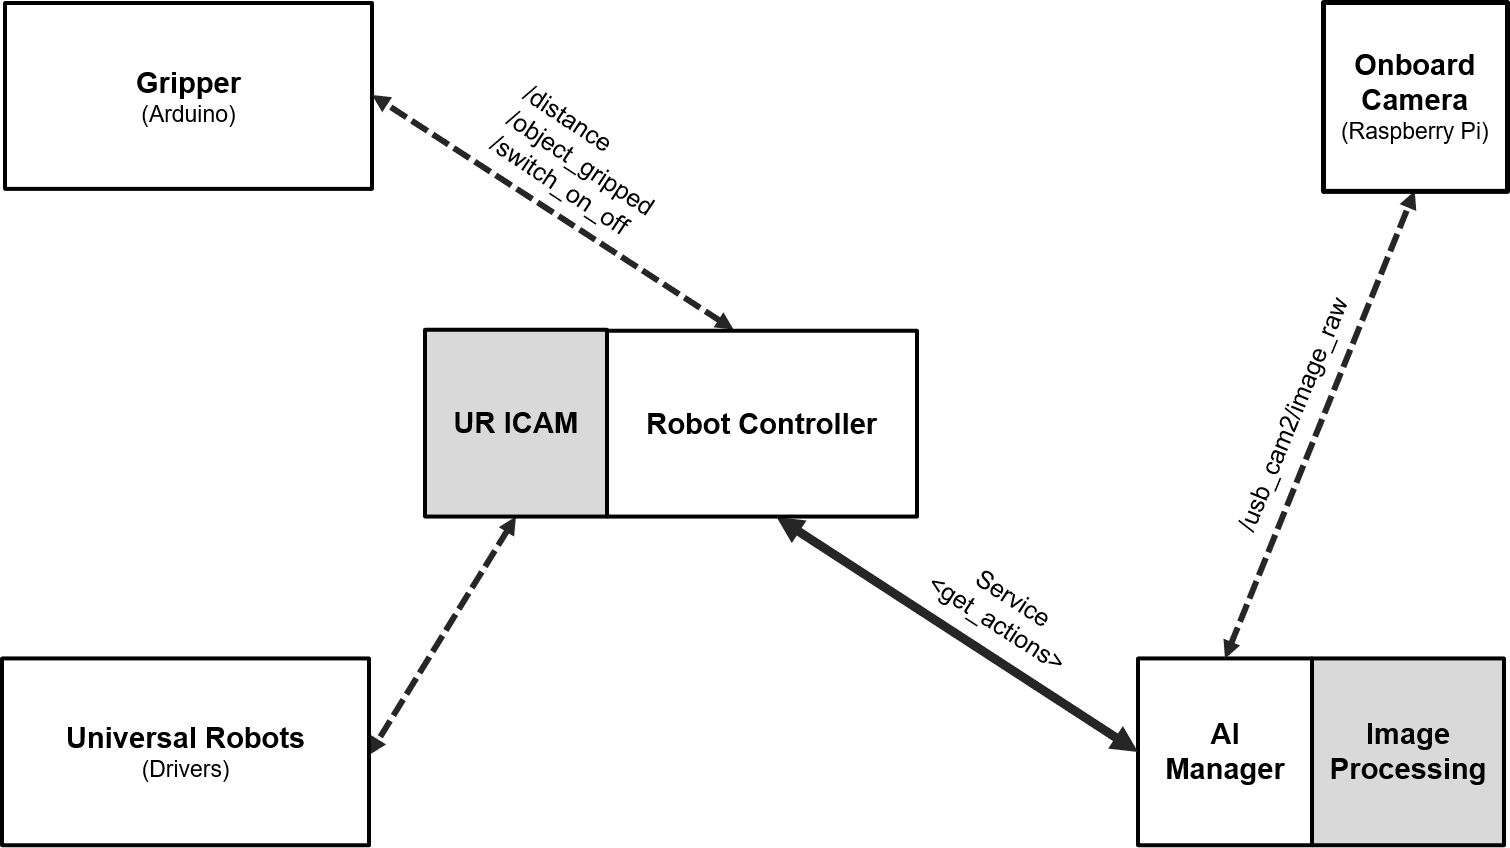
\includegraphics[width=0.7\linewidth]{Images/ArchitectureIV}
			\caption[Architecture IV]{From the simplest to the final Architecture IV}
			\label{fig:architectureiV}
		\end{figure}
	
		We commented before that AI Manager needs to gather a state image in order to start the training. To gather this image, it just requests a message from \textbf{\textendash \textit{usb\_cam\textendash image\_raw}} topic. Messages of this topic are published by Onboard Camera node, which is basically an instance of usb\_cam node that publishes with a 30 fps rate the images of the Onboard camera of the robot. 
		
		But once the Ai Manager has the image, it has to process it and extract its features, and Ai Manager will do it using the models in Image Processing. We will talk deeply about this later, but it basically means to make some transformation to the image (Changing its shape, color, rotation, etc. ) and pass it through a pre-trained Convolutional Neural Network in order to extract some features. This features are actually the ones that will be passed through the Reinforcement Learning Neural Network and the ones that will be stored in the Replay Memory.
		
		Finally, the last two nodes that we have not commented from \autoref{fig:architecture} are the Block Detector and the Upper Camera Node. Block Detector is a piece of code used by Robot Controller when it is performing a place action. In this moment, the robot is out of the box and has to decide the initial coordinates of the next episode. The upper camera has, though, a full view of the environment, so the Robot Controller takes the environment picture from the topic \textbf{\textendash \textit{usb\_cam2\textendash image\_raw}} where the Upper Camera node is publishing the images of the upper camera. Then it passes the image to the Block Detector which finally calculates the optimal point of return, avoiding the places of the box where there are no pieces.
		
		\begin{figure}[H]
			\centering
			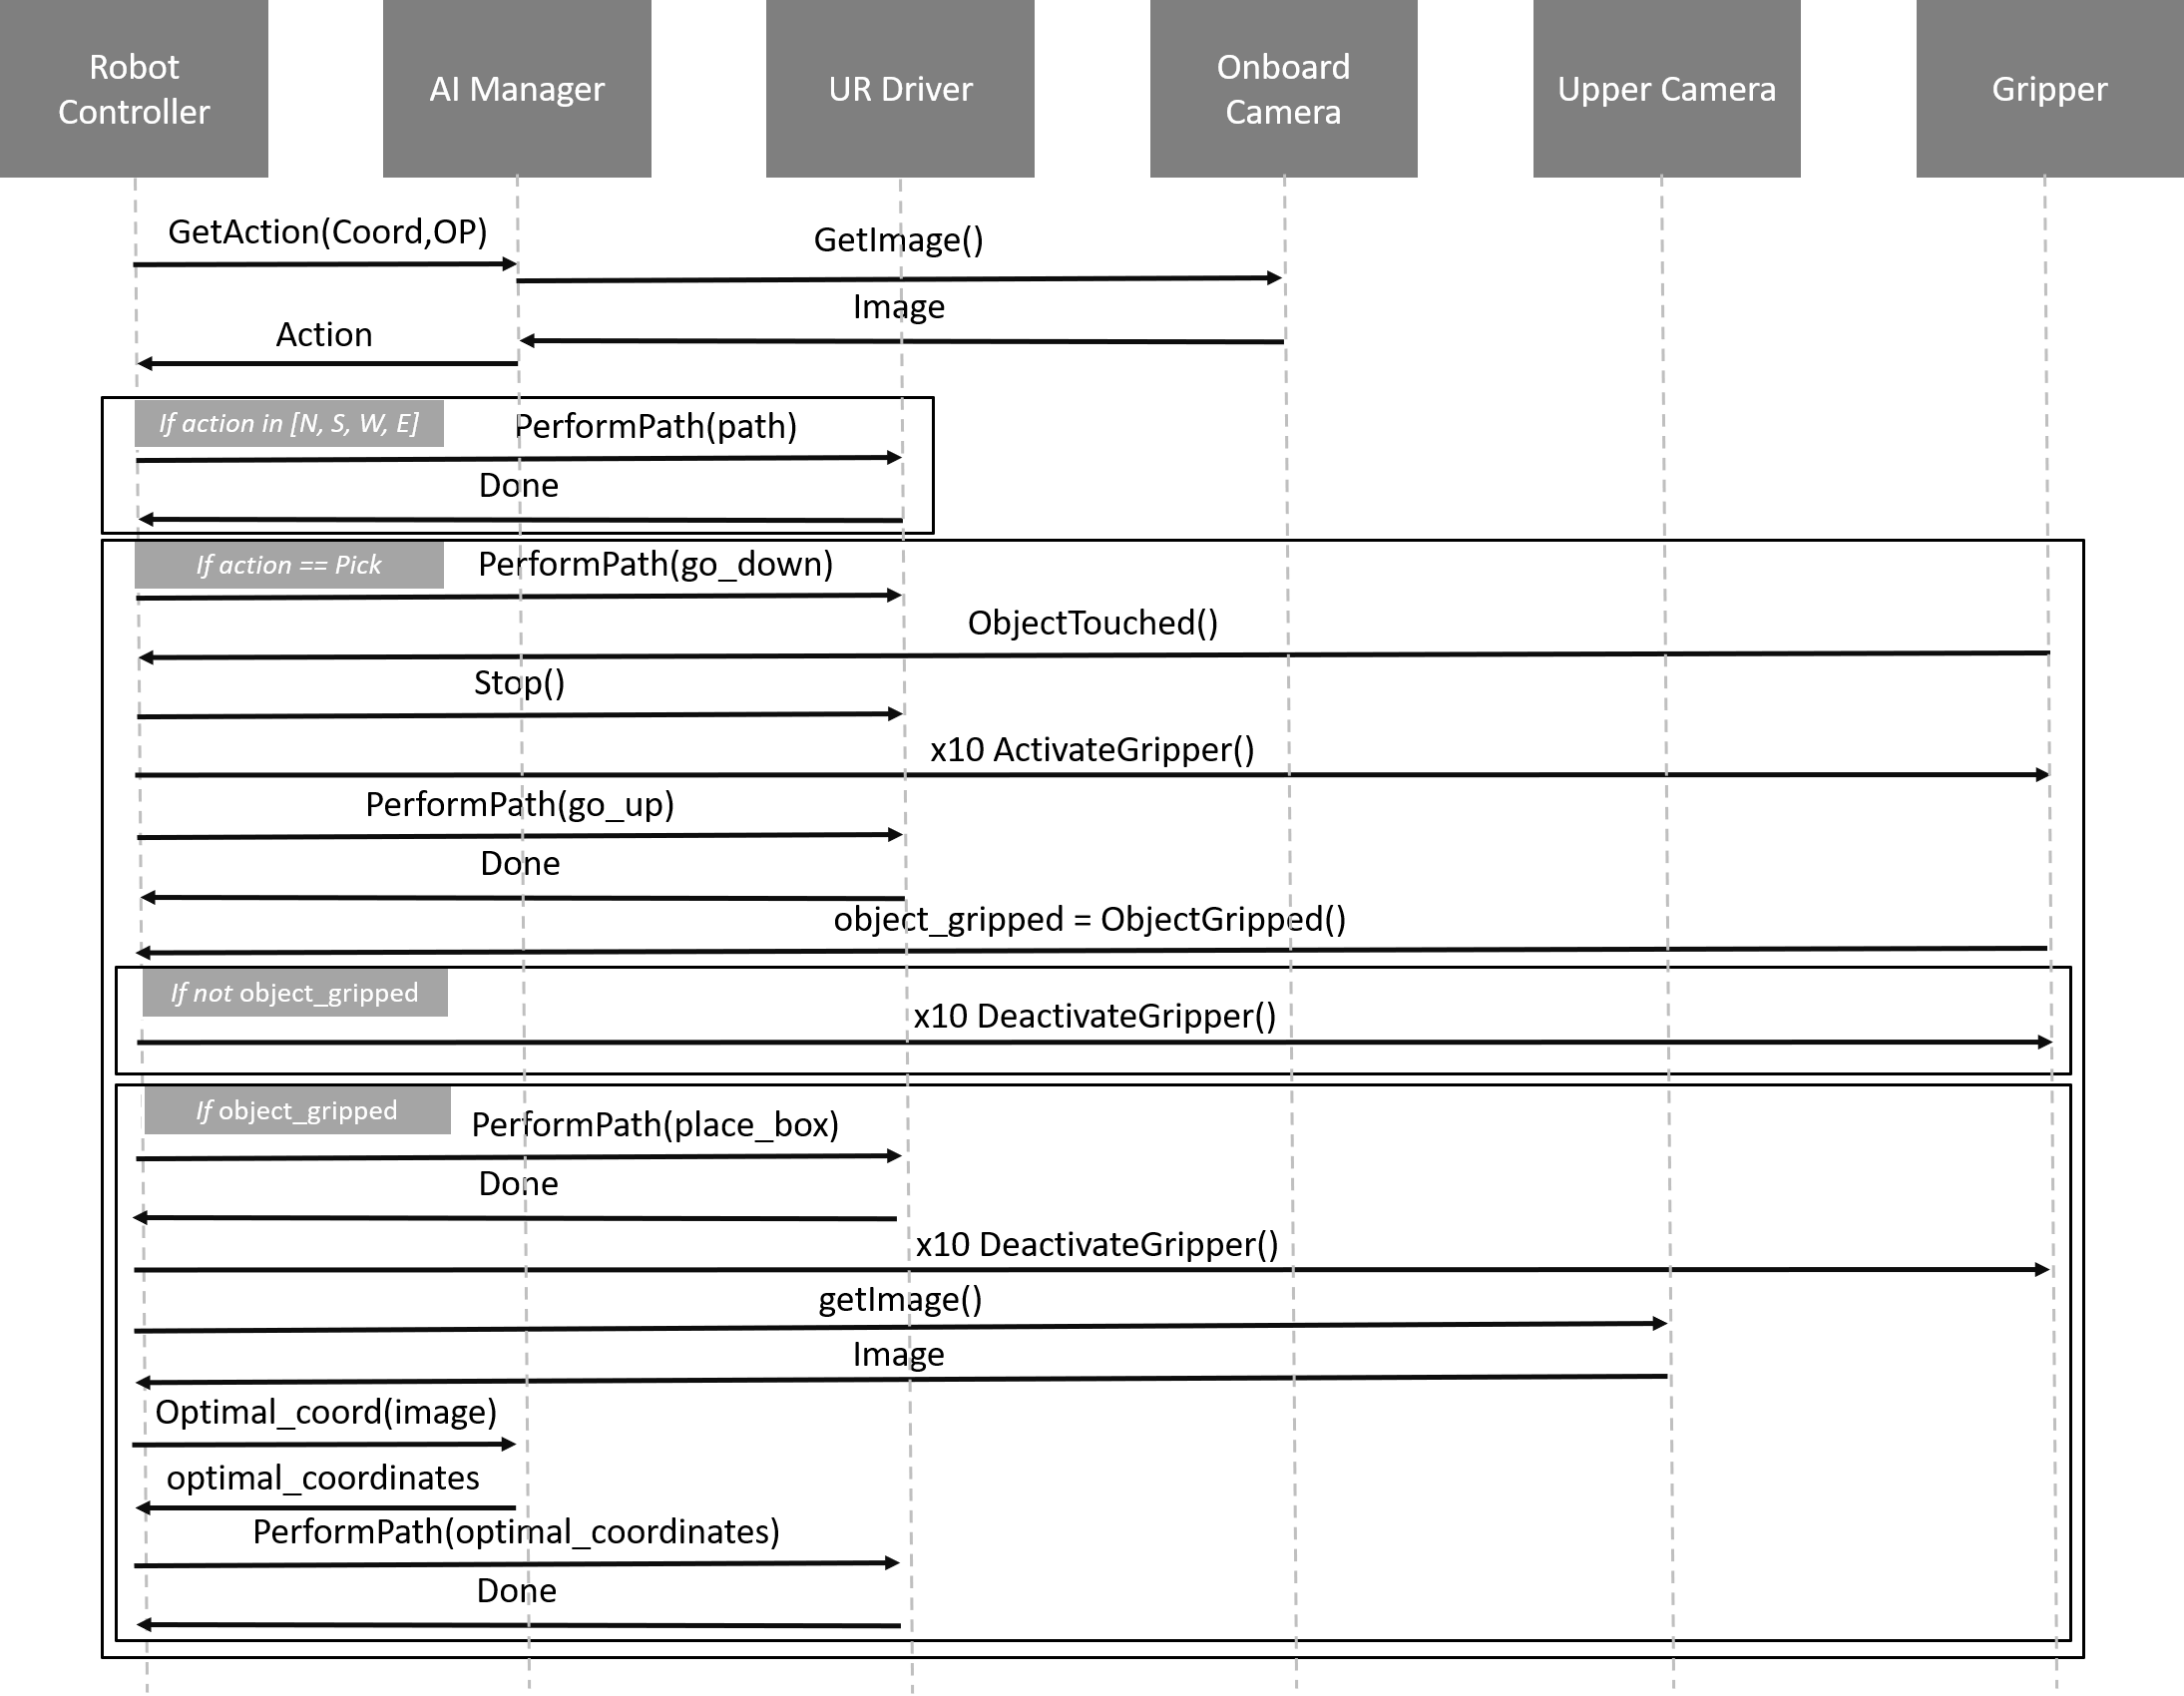
\includegraphics[width=1\linewidth]{Images/NodeInteraction}
			\caption[Node Interction]{Flow Chart of nodes interacting}
			\label{fig:nodeinteraction}
		\end{figure}
	
		To understand better all the architecture, in \autoref{fig:nodeinteraction} we can find a flow chart showing the iteration between nodes in one step. This flow would be in an infinite loop until the training is over. We can see how the step always starts with Robot Controller Asking AI Manager which action to perform, and AI Manager retrieving a picture from Onboard Camera to decide the action and train the Reinforcement Learning Algorithm. Behind this steps there is a complex process that we will talk about later.
		
		Then, depending on the action to perform, the flow would be really simple or more complex. If action is Pick, the robot has to start an asynchronous downward movement that will only be stopped once Robot Controller receive a True Message in the \textbf{\textit{\textbackslash distance }} topic, which means that the robot is now in contact with an object. Then, it will activate the gripper, go upwards to the original position and, if the robot has picked an object, perform a place action to put the object in the place box.
		
		This is a really simplified flow, but its a very good graphical way of understanding how the system works. To go deeply into the system, lets analyse each node separately:
		
		
	\section{ai\_manager}
	
			ai\_manager module is the "intelligence" of the robot, responsible for making it learn by training a Deep Reinforcement Learning Algorithm. Using this algorithm, the robot (\textbf{agent}) will explore the \textbf{Environment} by performing a set of \textbf{actions}. Once these actions are performed, the agent will receive a \textbf{reward} that can be positive, neutral or negative depending on how far the agent is from the objective.
			
			Each time the agent perform an action, it reaches a new \textbf{state}. States can be transitional or terminal, when the agent meets the objective or when it gets to a forbidden position. Each time the agent reaches a terminal state, an \textbf{episode} is ended, and a new one is started.
			
			The code of the AI Manager can be found in the appendix of this document, where a link to the github repository can also be found.
			
		\subsection{Definition of the problem}
			
			The objective of the agent is thus the first thing that has to be defined. In this case is simple: pick a piece.
			
			Then, the environment, the states and the actions have to be defined together. These decisions are conditioned by the hardware and materials available. In our case, as said before, we have a UR3 robot with six different points of movements, and a vacuum gripper. That means that the best way of griping an object is by facing the gripper to the floor and move it vertically until it gets in contact with the object, where the vacuum can be powered on, and we can know if the object has been griped or not.
			
			Having this in mind, we have decided that the robot have to be fixed in a specific height with the gripper facing down. Then, the actions will be "north", "south", "east" or "west" to move the robot through the x-y plane formed by these movements in the selected robot height, "pick", to perform the gripping process described before and place the object in the box, and "random\_state" to move the robot to a new random state when a terminal state is reached.
			
		\subsection{Environment.py}
			The environment is defined in Environment.py class. There, we can find different parameters and methods. All of them are explained in the code, but we will briefly explain them here. The CARTESIAN\_CENTER and the ANGULAR\_CENTER represent the same point in the space, but using different coordinates. This point should be the x-y center of the picking box with the robot height defined before as z point. As starting point, we need to use the ANGULAR\_CENTER because we want the robot to reach this point with the gripper facing down.
			
			Then, we have to define the edges of the box as terminal states, because we just want the robot to explore inside the box. To define those limits, we use X\_LENGTH and Y\_LENGTH parameters, which are the X and Y lengths of the box in cm.
			
			Other important parameters to define are the center of the box where we will place all the objects (PLACE\_CARTESIAN\_CENTER) or the distance that the robot has to move in each action (ACTION\_DISTANCE).
			
			Finally, the methods defined in this class are:
			
			\begin{itemize}
				\item[\textendash]\textbf{\textit{generate\_random\_state(strategy='ncc')}}, which is used when the agent reaches a terminal state and needs a new random state.
				\item[\textendash]\textbf{\textit{get\_relative\_corner(corner)}}, which returns the relative coordinates of a corner of the box
				\item[\textendash]\textbf{\textit{is\_terminal\_state(coordinates, object\_gripped)}}, which returns a boolean telling whether a given state is terminal or not using the parameters given.
			\end{itemize}
			
			
		\subsection{Rewards}
			Rewards are one of the most difficult-to-define parameters. In this case, rewards are deffined in the EnvManager inner class of RLAlgorithm.py. The specific value of the rewards are not given here because they are different from one training to another, but we give (positive or negative) rewards for:
			
			\begin{itemize}
				\item[\textendash]Terminal state after picking a piece.
				\item[\textendash]Terminal state after exceeding the box limits.
				\item[\textendash]Non terminal state after a pick action
				\item[\textendash]Other non terminal states
			\end{itemize}
			
		\subsection{Algorithm}
						
			This Deep Q Learning algorithm is implemented in the class RLAlgorithm.py following this schema:
			
			\begin{itemize}
				\item[\textendash]Initialize replay memory capacity.
				\item[\textendash]Initialize the policy network with random weights.
				\item[\textendash]Clone the policy network, and call it the target network.
				\item[\textendash]For each episode:
				\begin{itemize}
					\item[\textendash]Initialize the starting state.
					\item[\textendash]For each time step:
					\begin{itemize}
						\item[\textendash]Select an action via exploration or exploitation
						\item[\textendash]Execute selected action and observe reward and next state.
						\item[\textendash]Store experience in replay memory.
						\item[\textendash]Sample random batch from replay memory.
						\item[\textendash]Preprocess states from batch.
						\item[\textendash]Pass batch of preprocessed states to policy network.
						\item[\textendash]NN training. Weight back-propagation:
						\begin{itemize}
							\item[\textendash]Calculate loss between output Q-values and target Q-values.
							\item[\textendash]Using both the target and the policy networks to increase stability.
							\item[\textendash]Gradient descent updates weights in the policy network to minimize loss.
						\end{itemize}
						
					\end{itemize}
				\end{itemize}
				\item[\textendash]After X time steps or episodes, weights in the target network are updated to the weights in the policy network.
			\end{itemize}
		
			This schema is a little bit difficult to understand in the first moment, but it is deeply explained in the State of The Art section of this document.
			
			\subsubsection{RLAlgorithm.py}
				RLAlgorithm.py is the most important file of this module because it is the place where the algorithm implementation is done. Several classes have been used to implement the algorithm. Some of these classes are defined inside RLAlgorithm (inner classes) and others are normal outer classes.				
				In RLAlgorithm.py, we define the RLAlgorithm class, which also have several inner classes. These classes are:
				
				\begin{itemize}
					\item[\textendash]\textbf{Agent:} Inner class used to define the agent. The most important thing about this class is the select\_action method, which is the one used to calculate the action using whether Exploration or Exploitation.
					\item[\textendash]\textbf{DQN:} Inner class used to define the target and policy networks. It defines a neural network that have to be called using the vector of features calculated by passing the image through the feature extractor net.
					\item[\textendash]\textbf{EnvManager:} Inner Class used to manage the RL environment. It is used to perform actions such as calculate rewards or gather the current state of the robot. The most important methods are:
					\begin{itemize}
						\item[\textendash]\textbf{calculate\_reward}, which calculates the reward of each action depending on the initial and final state.
						\item[\textendash]\textbf{calculate\_reward}, which calculates the reward of each action depending on the initial and final state.
						\item[\textendash]\textbf{extract\_image\_features}, which is used to transform the image to extract image features by passing it through a pre-trained CNN network that can be found in ImageModel Module.
					\end{itemize}
					\item[\textendash]\textbf{EpsilonGreedyStrategy}: Inner Class used to perform the Epsilon greede strategy
					\item[\textendash]\textbf{QValues:} Inner class used to get the predicted q-values from the policy\_net for the specific state-action pairs passed in. States and actions are the state-action pairs that were sampled from replay memory.
					\item[\textendash]\textbf{ReplayMemory:} Inner Class used to create a Replay Memory for the RL algorithm
					\item[\textendash]\textbf{Environment:} Class where the RL Environment is defined
					\item[\textendash]\textbf{TrainingStatistics:} Class used to store all the training statistics. If it is run separately, It will plot a set of graphs to represent visually the training evolution.
					\item[\textendash]\textbf{ImageModel:} Class used to extract the image features used in the training. You can find this class in this repository, which store another module of this project.
					\item[\textendash]\textbf{ImageController:} Class used to gather and store the relative state images from a ros topic.
				\end{itemize}
				
				In order to implement the algorithm there are two important structures that are defined in the beginning of this file. These structures are:
				
				\begin{itemize}
					\item[\textendash]\textbf{State}, which defines all the things needed to represent a State:
					\begin{itemize}
						\item[\textendash]Coordinates of the robot.
						\item[\textendash]Image of the State. 
						\item[\textendash]Boolean telling if an object has been gripped.
					\end{itemize}
					\item[\textendash]\textbf{Experience}, which represents the experience of the agent in a given moment:
					\begin{itemize}
						\item[\textendash]The initial state of the agent (Image).
						\item[\textendash]The initial coordinates of the agent.
						\item[\textendash]The action taken by the agent.						
						\item[\textendash]The state reached after taking the action (Image).
						\item[\textendash]The coordinates reached after taking the action.
						\item[\textendash]The reward obtained for taking this action.
						\item[\textendash]Boolean telling whether the final state is terminal or not.
					\end{itemize}
				\end{itemize}
			
				Finally, there are some important methods in RLAlgorithm class that it is important to take into account to understand how this node works:
				
				\begin{itemize}
					\item[\textendash]\textbf{save\_training:} Method used to save the training so that it can be retaken later. It uses pickle library to do so and stores the whole RLAlgorithm object because all the context is needed to retake the training. This method also stores a pickle a TrainingStatistics object for them to be accessible easily.
					\item[\textendash]\textbf{recover\_training:} Method used to recover saved trainings. If it doesn't find a file with the name given, it creates a new RLAlgorithm object.
					\item[\textendash]\textbf{train\_net:} Method used to train both the train and target Deep Q Networks. We train the network minimizing the loss between the current Q-values of the action-state tuples and the target Q-values. Target Q-values are calculated using the Bellman's equation:
					\begin{gather*}
						q_*(s,a) = E[ R_t + \gamma max(q(s', a' )]
					\end{gather*}
					\item[\textendash]\textbf{next\_training\_step:} This method implements the Reinforcement Learning algorithm to control the UR3 robot. As the algorithm is prepared to be executed in real life, rewards and final states cannot be received until the action is finished, which is the beginning of next loop. Therefore, during an execution of this function, an action will be calculated and the previous action, its reward and its final state will be stored in the replay memory.
				\end{itemize}
			
			\subsection{Training Flow}
			
				